\documentclass[pdflatex,sn-mathphys-num,iicol]{sn-jnl}

\usepackage{amsmath,amssymb}
\usepackage{graphicx}
\usepackage{booktabs}
\usepackage{placeins}

\raggedbottom
\setlength{\textfloatsep}{12pt plus 2pt minus 2pt}
\setlength{\floatsep}{10pt plus 2pt minus 2pt}
\setlength{\intextsep}{10pt plus 2pt minus 2pt}

\begin{document}

\title[Cross-Dataset Generalization in Deepfake Detection]{Cross-Dataset Generalization in Deepfake Detection: A Controlled Study of Spatial, Frequency, and Video-Level Baselines}

\author*[1]{\fnm{Samarth} \sur{Kukreja}}\email{samarthkukreja2003@gmail.com}
\affil*[1]{\orgname{Independent Researcher}, \orgaddress{\city{Faridabad}, \state{Haryana}, \country{India}}}

\abstract{Deepfake detectors can report strong in-domain scores but still fail when the test videos come from a different dataset or if the videos are degraded by common image corruptions. I evaluate that gap with one fixed face-based pipeline and five ImageNet-pretrained red--green--blue (RGB) backbones: EfficientNet-B4, Xception, ResNet-50, ConvNeXt-Tiny, and Vision Transformer (ViT)-Base. The experiments use FaceForensics++ (FF++), Celeb-DF~(v2), and the DeepFake Detection (DFD) dataset in one source-video-disjoint in-distribution setting and three cross-dataset transfer settings. Metrics are computed at the video level by aggregating face-crop scores per source video, with accuracy, area under the receiver operating characteristic curve (AUC), F1 score, equal error rate (EER), bootstrap 95\% confidence intervals, and paired tests on the same held-out videos. I also add two low-cost probes: a score-level temporal aggregation baseline and a lightweight frequency-only ResNet-18 baseline. ConvNeXt-Tiny leads in Exp1, Exp2, and Exp4, but its advantage over ResNet-50 is not significant under the reported paired procedures in Exp1/Exp2 at this single training seed. The probes remain exploratory; Exp2 temporal transfer is confounded by different detector checkpoints. In these experiments, source-domain coverage and evaluation protocol matter at least as much as the backbone choice.}

\keywords{Deepfake detection, Cross-dataset generalization, Image processing, Video-level evaluation, Robustness, Neural networks}

\maketitle

\section{Introduction}
High validation accuracy on one deepfake benchmark was not enough for this project. The harder question was whether a source-trained detector would still separate real and fake videos on a different dataset. In practice that change may be a new manipulation method, a different identity pool, another compression pipeline, or a different source of real videos. Previous surveys and benchmarks have described this gap between in-distribution scores and cross-dataset reliability~\cite{ref1,ref:ffpp,ref:celebdf}, and I use it as the main focus of measurement here.

The models used here follow the common face-crop pipeline: sample frames, detect faces, classify each crop, and aggregate the crop scores back to the video. This approach does not include true temporal modeling, which recurrent and sequence-based detectors can use to capture motion cues that still-image models miss. That restriction is intentional because it lets the experiments ask a narrower question: when preprocessing and evaluation are fixed, how much does the image backbone itself matter under dataset shift?

The practical motivation is simple: a moderation or forensic system will rarely see the same distribution it was trained on. I address this concern in three ways: source videos are kept in separate splits, scores are reported at the video level, and point estimates are reported with uncertainty.

This is a controlled backbone study, not a new detector architecture. EfficientNet-B4, Xception, ResNet-50, ConvNeXt-Tiny, and ViT-Base share the same faces, splits, optimizer, augmentation policy, and video-level evaluation code. This design does not eliminate all sources of variance, especially because training uses a single seed, but it avoids changing multiple variables at the same time.

The study is organized around five questions. First, what happens when the usual FF++ experiment is made source-video-disjoint, with every crop from a video kept in the same split? Second, do source-trained detectors transfer when the source and target datasets differ: FF++$\to$Celeb-DF, Celeb-DF$\to$FF++, and mixed-source training$\to$DFD? Third, after using paired tests instead of raw rankings, do the five backbones separate into clear winners? Fourth, do two cheap add-ons---a frequency-only ResNet-18 and a score-level temporal classifier---change the cross-dataset pattern? Finally, which errors remain under manipulation-family breakdowns and common image corruptions?

The most relevant previous work uses RGB face crops. MesoNet works at a mesoscopic texture scale, and Face X-ray focuses on blending boundaries~\cite{ref:mesonet,ref:facexray}. Frequency cues provide different evidence from RGB texture: Frank et al. report generator traces in frequency space, and F$^3$-Net uses frequency-aware decompositions and local spectral statistics~\cite{ref:frank,ref:f3net}. Recurrent detectors and LipForensics instead use motion or mouth dynamics~\cite{ref2,ref:lipforensics}. More recent work continues to treat cross-domain generalization as a central challenge through latent-space augmentation, artifact attention, temporal style cues, and benchmark-wide evaluation~\cite{ref:lsda,ref:laanet,ref:styleflows,ref:gend}. I approach the problem from the evaluation side: source videos are separated, DFD remains held out in Exp4, and uncertainty is reported at the video level.

\section{Methodology}

The pipeline has four fixed stages. Videos are sampled into frames, then a multitask cascaded convolutional network (MTCNN)~\cite{ref:mtcnn} detects and crops faces. The resulting crops are assigned to leakage-controlled splits from the dataset manifests, and the selected backbone is fine-tuned with a binary classification head. At test time, crop-level scores are averaged within each source video, followed by computation of the evaluation metrics and bootstrap confidence intervals.

Frames are sampled every tenth frame. A face detection is retained only if its confidence is at least $0.95$ and the face box is at least 60 pixels on each side. The box is expanded by 20\%, cropped, resized, and filtered for blur; no more than 20 face crops are retained per video. All models receive $224\times224$ ImageNet-normalized red--green--blue (RGB) crops. Figure~\ref{fig:pipeline} summarizes the fixed workflow.

\begin{figure*}[!t]
\centering
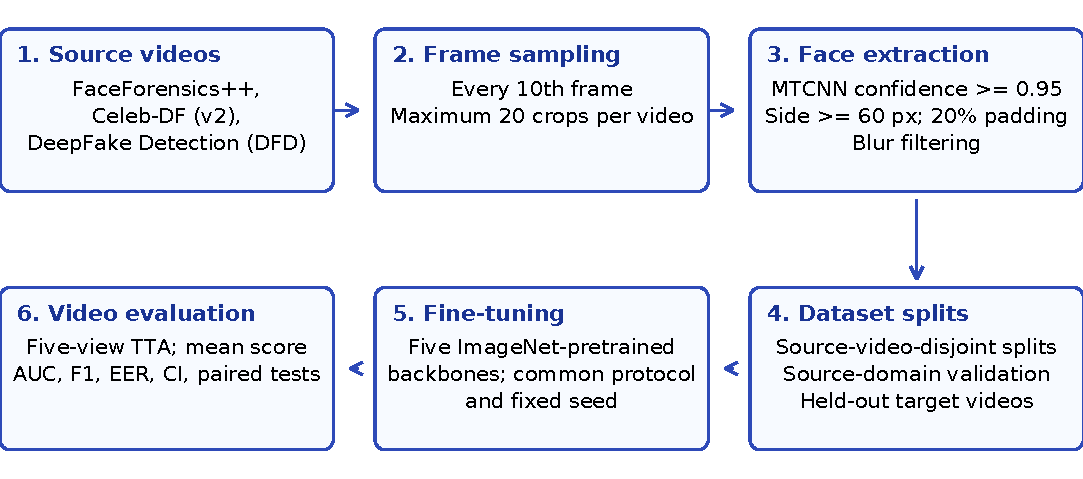
\includegraphics[width=0.95\textwidth]{Fig1.pdf}
\caption{Shared face-crop, training, and video-level evaluation pipeline}
\label{fig:pipeline}
\end{figure*}

The five backbones were selected as practical reference points rather than as new architectural designs. Xception is the classical FF++ reference, ResNet-50 is the standard residual baseline, EfficientNet-B4 is the efficiency-oriented baseline, ConvNeXt-Tiny is the modern convolutional neural network (CNN), and ViT-Base/16 is the transformer comparison~\cite{ref:xception,ref:resnet,ref:efficientnet,ref:convnext,ref:vit}. Each model is loaded with ImageNet-pretrained weights and uses a single-logit binary head.

The fine-tuning recipe is kept consistent across all backbones. It uses binary cross-entropy with logits and label smoothing $0.05$, AdamW learning rate and weight decay $10^{-4}$, cosine annealing, batch size 16 with four-step gradient accumulation, progressive unfreezing, and at most 30 epochs with patience 5 on source-domain validation area under the receiver operating characteristic curve (AUC). Random crop/resize, horizontal flip, mild colour jitter, rotation, and erasing are used only during training. Python, NumPy, and PyTorch share one fixed seed; deterministic cuDNN is enabled, and the resolved configurations and split identifiers are logged.

A video can contribute many similar face crops. To avoid counting those crops as independent test samples, I average the crop probabilities into one video score before computing the reported metrics. At inference, five-view test-time augmentation (TTA) averages the original crop, a horizontal flip, clockwise and counter-clockwise rotations, and a brightness-shifted view. Accuracy, AUC, F1 score, and equal error rate (EER) use a fixed threshold of $0.5$ where applicable. I calculate headline AUC confidence intervals with 1,000 video-level bootstrap resamples. Separately reported paired AUC analyses use 2,000 resamples of regenerated video scores; exact McNemar tests compare binary decisions on the same videos in Exp1 and Exp2, with Holm--Bonferroni adjustment. These analyses describe test-video uncertainty conditional on the saved trained models, not seed variance. The empirical bootstrap-tail convention and its limitations are documented in Online Resource~1.

\section{Experiments and Results}
\label{sec:experimental}
\subsection{Approach}
The evaluation has four settings: one source-video-disjoint in-domain FF++ run and three transfer runs. All headline RGB results use the same preprocessing, training recipe, and video-level metrics. The frequency and score-temporal probes are reported separately so they are not confused with the five-backbone comparison.

\subsection{Experimental Protocol}
\label{sec:protocol}
Table~\ref{tab:experiment_protocol} lists the split logic. Exp1 uses FF++ only, but it follows the official source-video partition: $720/140/140$ original videos for train/validation/test. A real video is assigned by its source-video identifier; a manipulated video is used only if both contributing source-video identifiers fall in the same split. Exp2 trains on FF++ and tests on Celeb-DF, Exp3 reverses that direction, and Exp4 trains on FF++ plus Celeb-DF before testing on DFD. Validation always comes from the training domain. Source-video separation does not establish person-identity disjointness.

\begin{table*}[!htbp]
\caption{Evaluation protocols. Validation is always source-domain; DFD is excluded from Exp4 training and validation. The FF++ collection includes 125/19 DeepFakeDetection-branch videos in Exp2 training/validation and 165 in Exp3 testing.}
\centering
\scriptsize
\setlength{\tabcolsep}{3pt}
\begin{tabular}{c l c c c}
\toprule
\textbf{Exp} & \textbf{Setting} & \textbf{Train} & \textbf{Val.} & \textbf{Test} \\
\midrule
1 & In-domain, source-video-disjoint & FF++ & FF++ & FF++ \\
2 & Cross-dataset & FF++ & FF++ & Celeb-DF \\
3 & Reverse transfer & Celeb-DF & Celeb-DF & FF++ \\
4 & Held-out domain & FF++ + Celeb-DF & FF++ + Celeb-DF & DFD \\
\botrule
\end{tabular}
\label{tab:experiment_protocol}
\end{table*}


\subsubsection{Leakage controls}
I check three possible leaks before training: FF++ source-video overlap in Exp1, video overlap across splits, and DFD leakage into the Exp4 training sources. All crops from a source video remain in one split, and FF++ entries from the ``DeepFakeDetection'' branch are excluded when DFD is used as the held-out test domain.

\subsubsection{Reproducibility settings}
The common settings are batch size~$16$, gradient accumulation over $4$ steps, effective batch size~$64$, at most $30$ epochs, patience~$5$, and AdamW learning rate/weight decay of $10^{-4}$. The exact graphics processing unit (GPU) and central processing unit (CPU) models were not preserved, so I do not report runtime or memory comparisons. The availability of retained code, configurations, split identifiers, and analysis scripts is stated below.


\subsubsection{Dataset Collection}
The experiments use three public datasets, each serving a different role in the transfer protocol. FF++ provides the source-video-disjoint in-domain split and the source side of Exp2; Celeb-DF is the Exp2 target and Exp3 source; DFD is the held-out target in Exp4. All crops from one video remain in one split. In Exp1, FF++ fake videos are retained only when both contributing source-video identifiers belong to the same partition, and DFD material is excluded from Exp4 training and validation. Class balancing is performed within each split.

Two additional probes build on the same saved faces and scores. The frequency probe converts each crop to a discrete cosine transform (DCT) log-magnitude input for a ResNet-18. The score-level temporal probe fits logistic regression to summary statistics of the saved crop scores, so it does not require another round of image training. Its Exp2 analysis uses Exp1 features for fitting and separately trained Exp2 detector features for testing; it is exploratory cross-checkpoint transfer. Corruption evaluation applies Joint Photographic Experts Group (JPEG) compression, Gaussian blur, additive noise, and downscale--upscale transformations without retraining. Online Resource~1 provides the complete result tables, statistical tests, ablations, failure analysis, robustness results, and leakage-control procedure.

\subsection{Results}
\label{sec:results}
Training of the five RGB backbones across the four main experiments is complete, with two additional probes reported below: a frequency-only ResNet-18 baseline and a no-retraining score-level temporal aggregation baseline. Unless stated, all reported values are video-level. Table~\ref{tab:main_auc} gives the primary AUC results; complete accuracy, F1, EER, confusion matrices, manipulation breakdowns, and pairwise-test tables appear in Online Resource~1.

\begin{table*}[!t]
\caption{Video-level AUC with 95\% bootstrap confidence intervals. Bold marks the highest point estimate in each experiment; it does not imply statistically significant superiority.}
\label{tab:main_auc}
\centering
\scriptsize
\setlength{\tabcolsep}{2pt}
\resizebox{\textwidth}{!}{%
\begin{tabular}{lcccc}
\toprule
Backbone & Exp1: FF++$\to$FF++ & Exp2: FF++$\to$Celeb-DF & Exp3: Celeb-DF$\to$FF++ & Exp4: Mixed$\to$DFD \\
\midrule
EfficientNet-B4 & 0.900 (0.85--0.94) & 0.713 (0.63--0.80) & 0.506 (0.47--0.54) & 0.788 (0.75--0.82) \\
Xception & 0.736 (0.65--0.81) & 0.573 (0.47--0.67) & 0.543 (0.51--0.57) & 0.735 (0.70--0.77) \\
ResNet-50 & 0.924 (0.88--0.97) & 0.799 (0.72--0.87) & \textbf{0.589 (0.56--0.62)} & 0.812 (0.78--0.84) \\
ConvNeXt-Tiny & \textbf{0.957 (0.92--0.99)} & \textbf{0.806 (0.72--0.88)} & 0.576 (0.54--0.61) & \textbf{0.915 (0.89--0.93)} \\
ViT-Base & 0.867 (0.80--0.93) & 0.668 (0.57--0.76) & 0.588 (0.56--0.62) & 0.713 (0.67--0.75) \\
\botrule
\end{tabular}%
}
\end{table*}

\subsubsection{Backbone comparison and transfer}
I read the numbers in Table~\ref{tab:main_auc} as point estimates first, then examine the reported paired comparisons, subject to the empirical bootstrap-tail limitations in Online Resource~1. ConvNeXt-Tiny and ResNet-50 have the two highest observed AUCs in Exp1, Exp2, and Exp4. Their difference is not significant after Holm adjustment in Exp1 ($q_{\mathrm{boot}}=0.147$, $q_{\mathrm{McN}}=0.688$) and is negligible in Exp2 ($\Delta\mathrm{AUC}=0.007$, $q_{\mathrm{boot}}=0.875$). I therefore report ConvNeXt-Tiny as the strongest observed point estimate, not as a uniquely superior architecture. ViT-Base does not lead under this common recipe. Because the five backbones share one baseline pipeline, the comparison should be read as a comparison under that recipe rather than as an optimization of each architecture's training strategy.

Every backbone degrades from the in-distribution setting to the cross-dataset settings, so the in-domain numbers overstate deployment performance. FF++$\to$Celeb-DF and Mixed$\to$DFD retain useful discrimination, whereas the reverse Celeb-DF$\to$FF++ transfer is weakest (AUC 0.506--0.589). ResNet-50's confidence interval in Exp3 lies above 0.5, so I describe this setting as weak or near-chance rather than uniformly at chance. Within this protocol, the asymmetry is consistent with source-domain coverage contributing to the result. However, dataset size, manipulation families, identities, and acquisition pipelines are confounded, so this interpretation should not be treated as a causal finding.

Figure~\ref{fig:generalization_summary} summarizes the cross-dataset means and the range across backbones for the four experiments.

\begin{figure*}[!t]
\centering
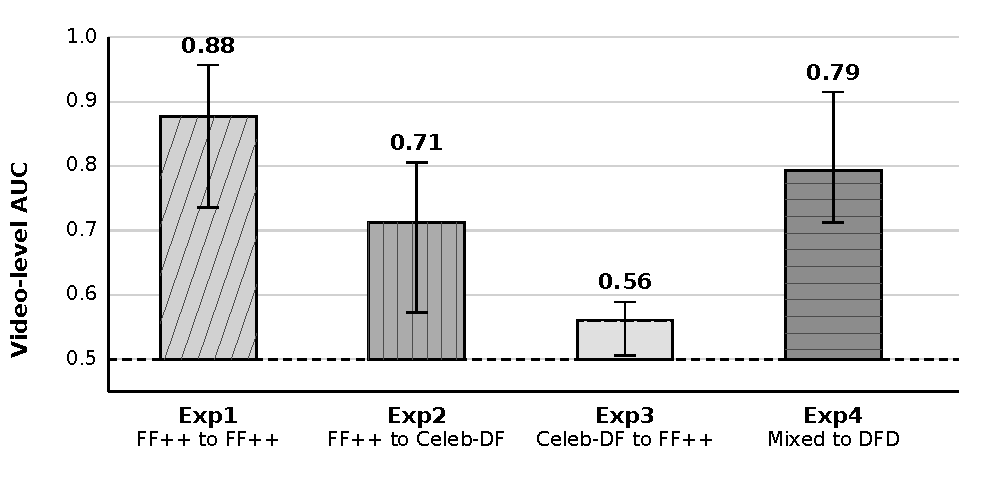
\includegraphics[width=0.92\textwidth]{Fig2.pdf}
\caption{Cross-dataset summary of Table~\ref{tab:main_auc}. Bars are means over the five backbones, whiskers show their minimum--maximum range, and the dashed line marks chance AUC}
\label{fig:generalization_summary}
\end{figure*}

\subsubsection{Diagnostic probes and robustness}
Table~\ref{tab:compact_diagnostics} keeps the diagnostic results most relevant to the central conclusion. The no-progressive-unfreezing configuration improves EfficientNet-B4 in every experiment; this comparison does not isolate freezing from the accompanying optimizer and learning-rate changes. I deliberately retain the common recipe in the headline comparison because only EfficientNet-B4 was ablated. Mean and median aggregation remain preferable to maximum/top-$k$ scoring. The frequency-only ResNet-18 carries some transfer signal in Exp2 but remains below the strongest RGB models, while logistic regression over score summaries does not consistently improve mean aggregation. The Exp2 temporal probe also changes detector checkpoint, so it does not isolate the effect of aggregation.

\begin{table*}[!t]
\caption{Selected diagnostic results (video-level AUC). ``Full'' is the EfficientNet-B4 baseline; frequency and temporal rows are auxiliary probes. Temporal Exp1 fits on 104 videos and evaluates on 45; its matched mean-score AUC is 0.823, not the 149-video headline value. Temporal Exp2 is exploratory cross-checkpoint transfer. Complete ablations are in Online Resource~1.}
\label{tab:compact_diagnostics}
\centering
\scriptsize
\setlength{\tabcolsep}{5pt}
\begin{tabular}{lcccc}
\toprule
Setting & Exp1 & Exp2 & Exp3 & Exp4 \\
\midrule
EfficientNet-B4 full & 0.900 & 0.713 & 0.506 & 0.788 \\
No progressive unfreezing & 0.927 & 0.812 & 0.546 & 0.813 \\
No training augmentation & 0.888 & 0.704 & 0.518 & 0.619 \\
No five-view TTA & 0.890 & 0.690 & 0.508 & 0.794 \\
Frequency-only ResNet-18 & 0.653 & 0.752 & -- & -- \\
Temporal-score probe (EfficientNet-B4) & 0.704 & 0.725 & -- & -- \\
\botrule
\end{tabular}
\end{table*}

To keep the corruption comparison clean, both the clean baseline and corrupted evaluations use single-view inference. Additive noise is the most damaging corruption, reducing AUC by 0.41, 0.23, and 0.30 in Exp1, Exp2, and Exp4 at the minimum observed AUC across tested severities. JPEG compression, blur, and downscaling also degrade performance, but their ordering varies by experiment. I read this as a measured robustness failure rather than a broad resilience result. Minimum-AUC summaries are supplied in Online Resource~1.

Overall, I treat this as an evaluation result rather than a new-detector claim. Backbone choice affects the observed point estimate, but source and target coverage, training choices, leakage control, and video-level evaluation materially affect the apparent generalization gap.


ConvNeXt-Tiny has the highest AUC point estimates in Exp1, Exp2, and Exp4. ResNet-50 comes second in those settings and remains close in the reported Exp1/Exp2 paired analyses. All backbones perform worse when assessed on a different dataset. The leakage controls and video-level uncertainty also matter when interpreting these results. Because every configuration was trained once with the same fixed seed, I do not treat the observed ranking as evidence of universal architectural superiority or run-to-run stability.

\section{Conclusion, Limitations and Future Work}
\subsection{Applications}
The detector can encounter videos which are different from those in the training set. This can happen in moderation, forensic triage, media-authenticity checks, or identity-verification procedures. I place more emphasis on transfer and held-out DFD testing than on FF++ in-domain accuracy alone.


\subsection{Conclusion}
Although ConvNeXt-Tiny leads in Exp1, Exp2, and Exp4, the reported adjusted Exp1/Exp2 procedures do not show a clear difference from ResNet-50. Outside the source distribution, performance drops for all five RGB backbones, and Celeb-DF$\to$FF++ remains close to chance level. The additional probes do not alter this picture. Frequency-only ResNet-18 retains some transfer ability despite poor in-domain performance, whereas score-level temporal features reduce AUC on the internal Exp1 split. Exp2 temporal results cannot isolate aggregation effects from the change in detector checkpoint. Because this is a controlled single-seed comparison, I do not identify a universally superior backbone.

The corruption tests reveal a similar limitation: predictions become less reliable when noise or blur is introduced on a detector trained on clean images. This analysis is intended as a diagnostic of the baseline pipeline rather than a comparative robustness benchmark across all five backbones.

\subsection{Limitations}
The main detectors operate at the frame level. The temporal probe only uses prediction statistics after inference, so it does not model temporal information directly. Exp2 combines dataset and detector-checkpoint changes; checkpoint binaries/hashes were unavailable for byte-level verification. The frequency experiment is also limited to a small ResNet-18 probe rather than a specialized detector such as F$^3$-Net, Face X-ray or LipForensics. The corruption study covers JPEG compression, blur, noise, and downscaling, but does not include adversarial attacks or platform-specific re-encoding. Each configuration was trained once with the same fixed seed because the available compute budget did not permit repeated training of all backbone--experiment combinations. The bootstrap intervals and paired tests therefore quantify uncertainty over held-out videos conditional on that trained model; they do not measure initialization, data-order, or optimization variability across seeds. The main backbone comparison also uses a common baseline training procedure rather than one individually optimized for each architecture. These constraints limit the conclusions to a controlled single-seed comparison and preclude claims of stable architectural ranking.

\subsection{Future Work (Requiring Training)}
Because the current study does not quantify run-to-run training stability, the next round of training should use multiple seeds. Future experiments could also evaluate a learned spectral or blending-boundary branch, a sequence model that uses temporal information directly instead of score statistics, and higher-resolution face crops if memory allows. More source and target datasets, such as the DeepFake Detection Challenge (DFDC) dataset~\cite{ref:dfdc}, would allow cross-dataset transfer to be evaluated across a wider range of dataset pairs.

\section*{Statements and Declarations}
\textbf{Funding.} The author received no specific funding for this work.

\textbf{Competing interests.} The author declares no competing interests.

\textbf{Author contributions.} Samarth Kukreja conceived the study, implemented the experiments, analysed the results, and wrote the manuscript.

\textbf{Artwork preparation.} Figures~1 and~2 were generated by the author in Python using ReportLab.

\textbf{Data and code availability.} FaceForensics++ and the Google/Jigsaw DeepFake Detection (DFD) dataset are available through the \href{https://github.com/ondyari/FaceForensics}{official FaceForensics++ repository and access procedure}; Celeb-DF~(v2) is available from its \href{https://github.com/yuezunli/celeb-deepfakeforensics}{official repository}. Access is subject to the respective dataset terms and approval procedures. The training and evaluation code, resolved configurations, dataset split identifiers/manifests, and video-level statistical-analysis scripts are available from the corresponding author on reasonable request.

\FloatBarrier

\begin{thebibliography}{99}

\bibitem{ref1} 
M. S. Rana, M. N. Nobi, B. Murali, and A. H. Sung, ``Deepfake Detection: A Systematic Literature Review,'' \textit{IEEE Access}, vol. 10, pp. 25494--25513, 2022, \url{https://doi.org/10.1109/ACCESS.2022.3154404}.

\bibitem{ref:ffpp}
A. R\"ossler, D. Cozzolino, L. Verdoliva, C. Riess, J. Thies, and M. Nie{\ss}ner, ``FaceForensics++: Learning to Detect Manipulated Facial Images,'' \textit{Proc. IEEE/CVF International Conference on Computer Vision (ICCV)}, 2019, pp. 1--11, \url{https://doi.org/10.1109/ICCV.2019.00009}.

\bibitem{ref:celebdf}
Y. Li, X. Yang, P. Sun, H. Qi, and S. Lyu, ``Celeb-DF: A Large-Scale Challenging Dataset for DeepFake Forensics,'' \textit{Proc. IEEE/CVF Conference on Computer Vision and Pattern Recognition (CVPR)}, 2020, pp. 3207--3216, \url{https://doi.org/10.1109/CVPR42600.2020.00327}.

\bibitem{ref:mesonet}
D. Afchar, V. Nozick, J. Yamagishi, and I. Echizen, ``MesoNet: a Compact Facial Video Forgery Detection Network,'' \textit{Proc. IEEE International Workshop on Information Forensics and Security (WIFS)}, 2018, pp.\ 1--7, \url{https://doi.org/10.1109/WIFS.2018.8630761}.

\bibitem{ref:facexray}
L. Li, J. Bao, T. Zhang, H. Yang, D. Chen, F. Wen, and B. Guo, ``Face X-ray for More General Face Forgery Detection,'' \textit{Proc. IEEE/CVF Conference on Computer Vision and Pattern Recognition (CVPR)}, 2020, pp.\ 5001--5010, \url{https://doi.org/10.1109/CVPR42600.2020.00505}.

\bibitem{ref:frank}
J. Frank, T. Eisenhofer, L. Sch\"onherr, A. Fischer, D. Kolossa, and T. Holz, ``Leveraging Frequency Analysis for Deep Fake Image Recognition,'' \textit{Proc. International Conference on Machine Learning (ICML)}, 2020, pp.\ 3247--3258.

\bibitem{ref:f3net}
Y. Qian, G. Yin, L. Sheng, Z. Chen, and J. Shao, ``Thinking in Frequency: Face Forgery Detection by Mining Frequency-aware Clues,'' \textit{Proc. European Conference on Computer Vision (ECCV)}, 2020, pp.\ 86--103, \url{https://doi.org/10.1007/978-3-030-58610-2_6}.

\bibitem{ref2}
D. G\"uera and E. J. Delp, ``Deepfake Video Detection Using Recurrent Neural Networks,'' 2018 15th IEEE International Conference on Advanced Video and Signal Based Surveillance (AVSS), Auckland, New Zealand, 2018, pp. 1--6, \url{https://doi.org/10.1109/AVSS.2018.8639163}.

\bibitem{ref:lipforensics}
A. Haliassos, K. Vougioukas, S. Petridis, and M. Pantic, ``Lips Don't Lie: A Generalisable and Robust Approach to Face Forgery Detection,'' \textit{Proc. IEEE/CVF Conference on Computer Vision and Pattern Recognition (CVPR)}, 2021, pp.\ 5039--5049, \url{https://doi.org/10.1109/CVPR46437.2021.00500}.

\bibitem{ref:lsda}
Z. Yan, Y. Luo, S. Lyu, Q. Liu, and B. Wu, ``Transcending Forgery Specificity with Latent Space Augmentation for Generalizable Deepfake Detection,'' \textit{Proc. IEEE/CVF Conference on Computer Vision and Pattern Recognition (CVPR)}, 2024, pp. 8984--8994, \url{https://doi.org/10.1109/CVPR52733.2024.00858}.

\bibitem{ref:laanet}
D. Nguyen, N. Mejri, I. P. Singh, P. Kuleshova, M. Astrid, A. Kacem, E. Ghorbel, and D. Aouada, ``LAA-Net: Localized Artifact Attention Network for Quality-Agnostic and Generalizable Deepfake Detection,'' \textit{Proc. IEEE/CVF Conference on Computer Vision and Pattern Recognition (CVPR)}, 2024, pp. 17395--17405, \url{https://doi.org/10.1109/CVPR52733.2024.01647}.

\bibitem{ref:styleflows}
J. Choi, T. Kim, Y. Jeong, S. Baek, and J. Choi, ``Exploiting Style Latent Flows for Generalizing Deepfake Video Detection,'' \textit{Proc. IEEE/CVF Conference on Computer Vision and Pattern Recognition (CVPR)}, 2024, pp. 1133--1143, \url{https://doi.org/10.1109/CVPR52733.2024.00114}.

\bibitem{ref:gend}
A. Yermakov, J. Cech, J. Matas, and M. Fritz, ``Deepfake Detection that Generalizes Across Benchmarks,'' \textit{Proc. IEEE/CVF Winter Conference on Applications of Computer Vision (WACV)}, 2026, \url{https://doi.org/10.1109/WACV61042.2026.00082}.

\bibitem{ref:mtcnn}
K. Zhang, Z. Zhang, Z. Li, and Y. Qiao, ``Joint Face Detection and Alignment Using Multitask Cascaded Convolutional Networks,'' \textit{IEEE Signal Processing Letters}, vol. 23, no. 10, pp. 1499--1503, 2016, \url{https://doi.org/10.1109/LSP.2016.2603342}.

\bibitem{ref:xception}
F. Chollet, ``Xception: Deep Learning with Depthwise Separable Convolutions,'' \textit{Proc. IEEE Conference on Computer Vision and Pattern Recognition (CVPR)}, 2017, pp. 1251--1258, \url{https://doi.org/10.1109/CVPR.2017.195}.

\bibitem{ref:resnet}
K. He, X. Zhang, S. Ren, and J. Sun, ``Deep Residual Learning for Image Recognition,'' \textit{Proc. IEEE Conference on Computer Vision and Pattern Recognition (CVPR)}, 2016, pp. 770--778, \url{https://doi.org/10.1109/CVPR.2016.90}.

\bibitem{ref:efficientnet}
M. Tan and Q. V. Le, ``EfficientNet: Rethinking Model Scaling for Convolutional Neural Networks,'' \textit{Proc. International Conference on Machine Learning (ICML)}, 2019, pp. 6105--6114.

\bibitem{ref:convnext}
Z. Liu, H. Mao, C.-Y. Wu, C. Feichtenhofer, T. Darrell, and S. Xie, ``A ConvNet for the 2020s,'' \textit{Proc. IEEE/CVF Conference on Computer Vision and Pattern Recognition (CVPR)}, 2022, pp. 11976--11986, \url{https://doi.org/10.1109/CVPR52688.2022.01167}.

\bibitem{ref:vit}
A. Dosovitskiy et al., ``An Image is Worth 16$\times$16 Words: Transformers for Image Recognition at Scale,'' \textit{Proc. International Conference on Learning Representations (ICLR)}, 2021.

\bibitem{ref:dfdc}
B. Dolhansky, J. Bitton, B. Pflaum, J. Lu, R. Howes, M. Wang, and C. C. Ferrer, ``The DeepFake Detection Challenge (DFDC) Dataset,'' \textit{arXiv preprint arXiv:2006.07397}, 2020, \url{https://doi.org/10.48550/arXiv.2006.07397}.

\end{thebibliography}

\end{document}
